\begin{exercise}{Propagation dans un réseau de ballons}{2}{Spé}
{Propagation}{lelay, centrale}

\begin{questions}
    \questioncours Loi des gaz parfaits, loi de Laplace pour une transformation isentropique.
    \question On considère un ballon de volume $V_0$ rempli d'un gaz parfait de coefficient $\gamma$ ouvert sur un tube de section $s$ à l'intérieur duquel peut coulisser sans frottements un piston de masse $m$, comme représenté sur le schéma ci dessous.
    \begin{center}
    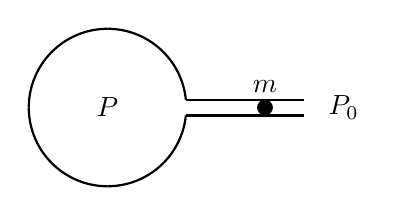
\begin{tikzpicture}
        % circle
        \draw[thick] (0, 1) arc ( 90: 180:1);
        \draw[thick] (0, 1) arc ( 90: 5.7:1);
        \draw[thick] (0,-1) arc (-90:-5.7:1);
        \draw[thick] (0,-1) arc (-90:-180:1);
        % right
        \draw[thick] ( 1, 0.1) -- (2.5,0.1);
        \draw[thick] ( 1,-0.1) -- (2.5,-0.1);
        \fill[black] (2,0) circle (0.1) node[above=2pt] {$m$};
        \draw (0,0) node[anchor=center] {$P$};
        \draw (3,0) node[anchor=center] {$P_0$};
    \end{tikzpicture}
    \end{center}
    \begin{parts}
        \part Sous quelle condition sur $P$ le piston est-il à l'équilibre ?
        \part En $t=0$, le piston est éloigné de sa position d'équilibre d'une quantité $\xi_0$. Établir l'équation du mouvement du piston dans l'hypothèse d'une évolution adiabatique et réversible du gaz.
        \part Dans l'approximation d'un petit déplacement, résoudre cette équation et donner $\xi(t)$.
    \end{parts}
    \question On considère maintenant un assemblage de $N \gg 1$ ballons tels que celui décrit précédemment, chacun étant relié au suivant par un tube de section $s$ dans lequel coulisse un piston $m$. À l'équilibre, les masses $m$ sont placées en $x = na$ avec $n \in \mathbb{Z}$, et on note $\xi_n$ le déplacement par rapport à sa position d'équilibre de la $n$-ième masse.
    \begin{center}
    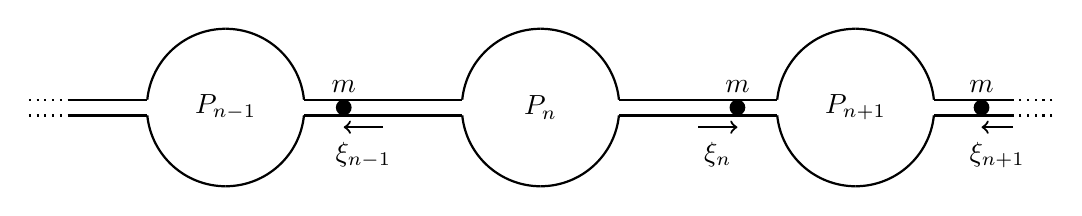
\begin{tikzpicture}
    % CENTRE = 0
        \draw (0,0) node[anchor=center] {$P_n$};
        % circle
        \draw[thick] (0, 1) arc ( 90: 174.3:1);
        \draw[thick] (0, 1) arc ( 90:   5.7:1);
        \draw[thick] (0,-1) arc (-90:  -5.7:1);
        \draw[thick] (0,-1) arc (-90:-174.3:1);
        % left
        \draw[thick] (-1, 0.1) -- (-2, 0.1);
        \draw[thick] (-1,-0.1) -- (-2,-0.1);
        % right
        \draw[thick] ( 1, 0.1) -- (2,0.1);
        \draw[thick] ( 1,-0.1) -- (2,-0.1);
    % CENTRE = 4
        \draw (4,0) node[anchor=center] {$P_{n+1}$};
        % circle
        \draw[thick] (4, 1) arc ( 90: 174.3:1);
        \draw[thick] (4, 1) arc ( 90:   5.7:1);
        \draw[thick] (4,-1) arc (-90:  -5.7:1);
        \draw[thick] (4,-1) arc (-90:-174.3:1);
        % left
        \draw[thick] (-1+4, 0.1) -- (-2+4, 0.1);
        \draw[thick] (-1+4,-0.1) -- (-2+4,-0.1);
        % right
        \draw[thick] ( 1+4, 0.1) -- (2+4,0.1);
        \draw[thick] ( 1+4,-0.1) -- (2+4,-0.1);
    % CENTRE = -4
        \draw (-4,0) node[anchor=center] {$P_{n-1}$};
        % circle
        \draw[thick] (-4, 1) arc ( 90: 174.3:1);
        \draw[thick] (-4, 1) arc ( 90:   5.7:1);
        \draw[thick] (-4,-1) arc (-90:  -5.7:1);
        \draw[thick] (-4,-1) arc (-90:-174.3:1);
        % left
        \draw[thick] (-1-4, 0.1) -- (-2-4, 0.1);
        \draw[thick] (-1-4,-0.1) -- (-2-4,-0.1);
        % right
        \draw[thick] ( 1-4, 0.1) -- (2-4,0.1);
        \draw[thick] ( 1-4,-0.1) -- (2-4,-0.1);
    % END LEFT
        \draw[dotted, thick] (-2.5-4, 0.1) -- (-2-4, 0.1);
        \draw[dotted, thick] (-2.5-4,-0.1) -- (-2-4,-0.1);
    % END RIGHT
        \draw[dotted, thick] (2.5+4, 0.1) -- (2+4, 0.1);
        \draw[dotted, thick] (2.5+4,-0.1) -- (2+4,-0.1);
    % MASSES
        \fill[black] (2.5,0) circle (0.1) node[above=2pt] {$m$};
        \draw[->, thick] (2,-0.25) -- (2.5,-0.25);
        \draw (2.25,-0.25) node[below=2pt] {$\xi_n$};
        \fill[black] (-2.5,0) circle (0.1) node[above=2pt] {$m$};
        \draw[->, thick] (-2,-0.25) -- (-2.5,-0.25);
        \draw (-2.25,-0.25) node[below=2pt] {$\xi_{n-1}$};
        \fill[black] (5.6,0) circle (0.1) node[above=2pt] {$m$};
        \draw[->, thick] (6,-0.25) -- (5.6,-0.25);
        \draw (5.8,-0.25) node[below=2pt] {$\xi_{n+1}$};
    \end{tikzpicture}
    \end{center}
    Donner l'équation d'évolution de $\xi_n$ pour un $n$ quelconque au premier ordre.
    \uplevel{On envisage la propagation d'une OPPH, et on propose donc d'écrire les $\xi_n$ sous la forme}
    \begin{align*}
        \xi_n = A e^{j(\omega t - k n a)}
    \end{align*}
    \question L'onde mécanique étudiée est-elle longitudinale ou transverse ? Quel(s) autre(s) type d'ondes de la même catégorie connaissez-vous ?
    \question On suppose $\lambda \ll a$. Transformer l'équation du mouvement des masses pour faire apparaître une équation de d'Alembert unidimensionnelle. Donner l'expression de la célérité $c$ correspondante.
    \question Si on suppose que les ballons sont en fait des tubes de section $s$ et qu'on a donc $V_0 = sa$, donner la nouvelle expression de la célérité $c$. En faire une application numérique pour l'air. Commenter
\end{questions}

\end{exercise}